% Wafer-level heat path (TikZ): large die grid + backside global cooling
% (uniform grounded g_vert) + lateral face adjacency through the
% interposer/substrate plane. Every branch carries its physical path type
% + value provenance; nodes carry role/size. All routing orthogonal;
% sans-serif.
%
% Sources: thermal-module-catalog Sec 3 (g_vert = h_cooling*A, water
% cooling h ~ 1e3-1e4 W/m2K standard magnitude; lateral conduction
% k*A/L through the interposer plane). Numeric h not fabricated.
\documentclass[border=10pt]{standalone}
\usepackage{sfmath}
\renewcommand{\familydefault}{\sfdefault}
\usepackage{tikz}
\usetikzlibrary{arrows.meta, shapes.geometric}
\definecolor{diefill}{HTML}{E8F0FE}
\definecolor{dieedge}{HTML}{1A73E8}
\definecolor{bndfill}{HTML}{F1F3F4}
\definecolor{bndedge}{HTML}{5F6368}
\definecolor{latedge}{HTML}{9334E6}   % lateral face adjacency: purple
\definecolor{gvedge}{HTML}{188038}    % backside g_vert: green
\begin{document}
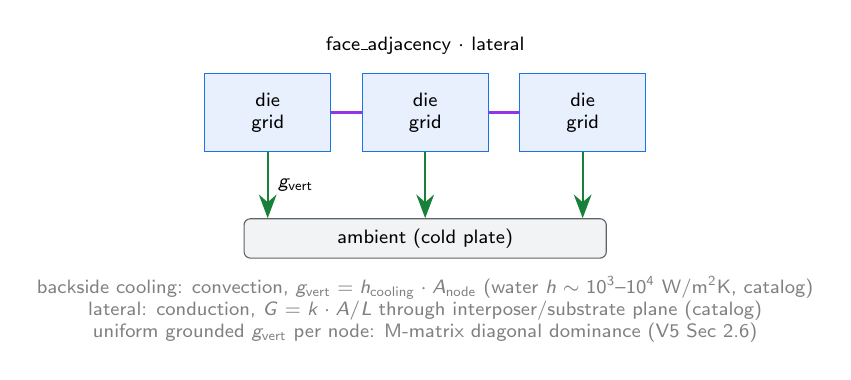
\begin{tikzpicture}[
  die/.style={rectangle, draw=dieedge, fill=diefill, minimum width=1.6cm,
              minimum height=1.0cm, align=center, font=\scriptsize},
  bnd/.style={rectangle, rounded corners=0.08cm, draw=bndedge, fill=bndfill,
              minimum width=4.6cm, minimum height=0.5cm, align=center, font=\scriptsize},
  lat/.style={draw=latedge, thick},
  gv/.style={draw=gvedge, thick, -{Stealth[length=3mm]}},
  lab/.style={font=\scriptsize},
]
% ---- die grid (1x3 schematic of the large grid) ----
\node[die] (d0) at (-2.0, 0.0) {die\\grid};
\node[die] (d1) at ( 0.0, 0.0) {die\\grid};
\node[die] (d2) at ( 2.0, 0.0) {die\\grid};
% ---- lateral face adjacency (interposer/substrate plane) ----
\draw[lat] (d0.east) -- (d1.west);
\draw[lat] (d1.east) -- (d2.west);
\node[lab] at (0, 0.85) {face\_adjacency $\cdot$ lateral};
% ---- backside global cooling: every die -> g_vert -> cold-plate ambient ----
\node[bnd] (coldplate) at (0, -1.6) {ambient (cold plate)};
\draw[gv] (d0.south) -- node[right, lab] {$g_{\mathrm{vert}}$} (d0.south |- coldplate.north);
\draw[gv] (d1.south) -- (d1.south |- coldplate.north);
\draw[gv] (d2.south) -- (d2.south |- coldplate.north);
% branch annotation: physical path type + value provenance (3 lines)
\node[lab, align=center, text=gray] at (0, -2.5) {
  backside cooling: convection, $g_{\mathrm{vert}}=h_{\mathrm{cooling}} \cdot A_{\mathrm{node}}$ (water $h \sim 10^3$--$10^4$ W/m$^2$K, catalog)\\
  lateral: conduction, $G=k \cdot A/L$ through interposer/substrate plane (catalog)\\
  uniform grounded $g_{\mathrm{vert}}$ per node: M-matrix diagonal dominance (V5 Sec 2.6)};
\end{tikzpicture}
\end{document}
